\begin{figure}[t]
    \centering
    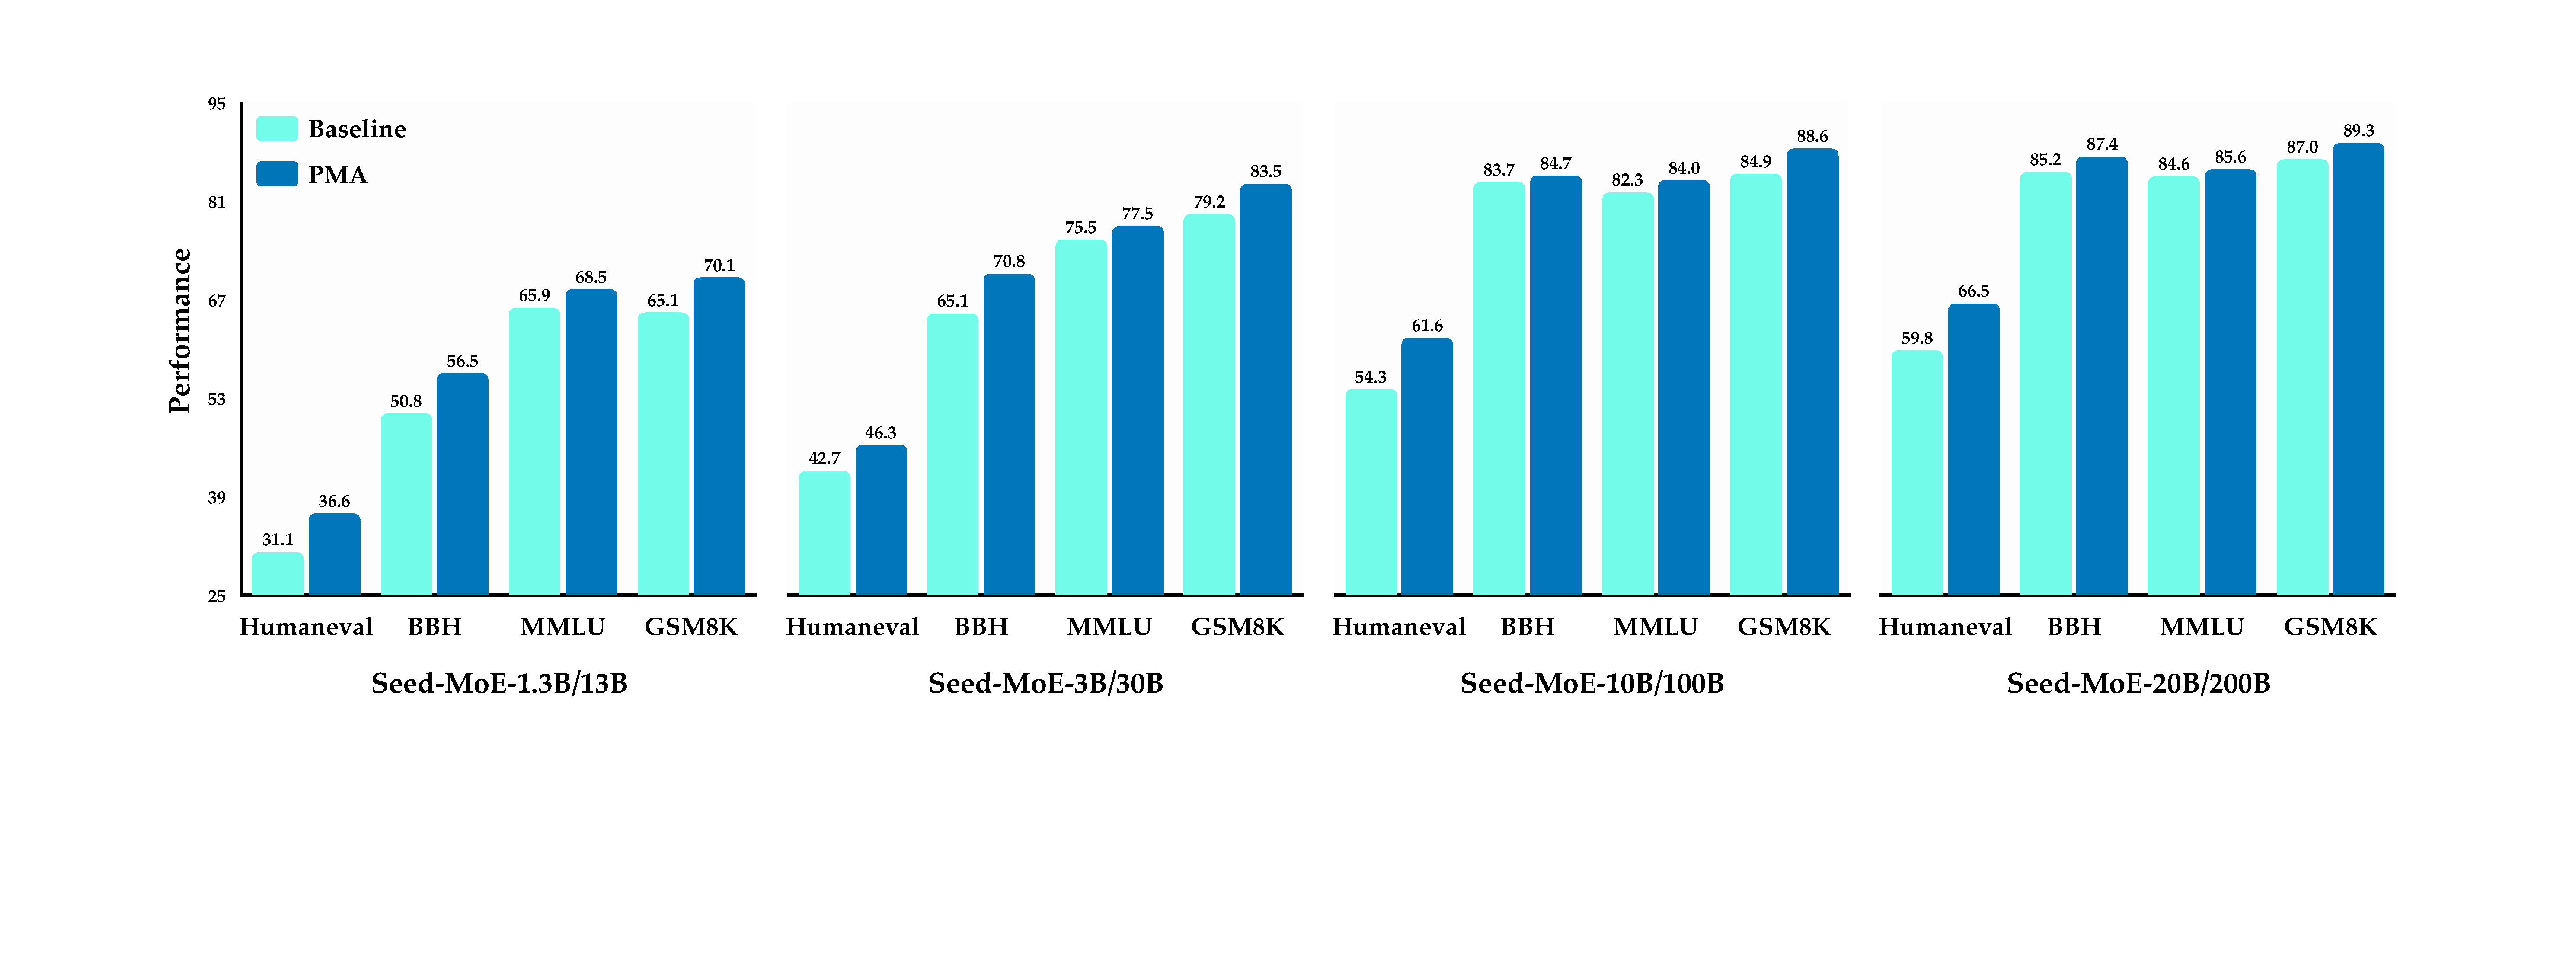
\includegraphics[width=1\linewidth]{image/overall.pdf}
    \caption{Comparison of downstream task performance for MoE models of varying sizes under stable training, before and after model merging.}
    \label{fig:overall}
\end{figure}
\section{Related Work}
Model merging is an emerging field undergoing rapid development, with diverse applications across various domains. Typically, model merging is implemented during the \textbf{post-training} phase~\citep{ilharco2022editing,zhou2024metagpt,yu2024language}, where multiple models fine-tuned on different downstream tasks are combined by merging their weights. This process effectively integrates the distinct capabilities of each individual model, resulting in a unified model that exhibits robust and comprehensive performance.

Recently, several methods have advanced this field significantly. For instance, Task Arithmetic~\citep{ilharco2022editing}, Ties-Merging~\citep{yadav2023resolving}, and AdaMerging~\citep{yang2023adamerging} integrate Vision Transformer (ViT) models~\citep{dosovitskiy2020image} trained on distinct visual classification tasks, producing a single model capable of multi-task object classification. PAPA~\citep{jolicoeur2023population} integrates the broad applicability of ensembling with the computational efficiency of weight averaging. MetaGPT~\citep{zhou2024metagpt} frames model merging as a multi-task learning problem, aiming to minimize the average loss between the merged model and individual task-specific models. Fisher Merging~\citep{matena2022merging} employs a weighted fusion of model parameters, with weights determined by the Fisher information matrix. RegMean~\citep{jin2022dataless} elegantly addresses the merging process by formulating it as a linear regression problem solvable through closed-form solutions. Evolutionary-model-merge~\citep{akiba2025evolutionary} efficiently optimizes merging coefficients using evolutionary algorithms. Additionally, DARE~\citep{yu2024language} merges multiple task-specific language models into a versatile unified model by randomly dropping and subsequently rescaling the delta parameters.

However, research on model merging during the \textbf{pre-training} phase remains relatively limited. Such studies typically refer to incorporating checkpoints within a single training trajectory during large language model (LLM) pre-training.
For example, LAWA~\citep{kaddour2022stop,hagele2024scaling,li2022trainable} demonstrated that merging checkpoints at intermediate stages can significantly accelerate training. Sanyal et al.~\citep{sanyal2023early} further indicated that checkpoint averaging combined with a high learning rate in pre-training trajectories contributes to faster convergence. Additionally, Checkpoint Merging~\citep{liu2024checkpoint} provided a comprehensive evaluation of the effectiveness of merging checkpoints at different stages during the pre-training of the Baichuan2~\citep{yang2023baichuan} LLM. Furthermore, technical reports of large-scale models such as Deepseek V3~\citep{liu2024deepseek} and LLaMA3.1~\citep{grattafiori2024llama} also mention the use of model merging techniques during pre-training, although detailed methodologies have not been publicly disclosed.
This paper primarily explores techniques for model merging within the pre-training paradigm. To the best of our knowledge, this is the first study to provide detailed technical insights into scaling model merging methods to significantly larger model sizes. We also discuss practical approaches for effective model merging and analyze its potential capabilities as well as its limitations.
%\subsection{Hello World}